\documentclass[a4paper]{article}
\usepackage[utf8]{inputenc}
\usepackage{graphicx}
\usepackage[citestyle=authoryear]{biblatex}
%\bibliographystyle{apalike}
\usepackage{rotating}
\addbibresource{mendeley.bib}
\usepackage{indentfirst}
\usepackage[margin = 1 in]{geometry}
\usepackage{xcolor}
\usepackage{wrapfig}

\title{Dissertation Outline}
\author{S. Katie Fogg}


\begin{document}
\maketitle

\section*{Overview}
Floodplain stream reaches have expansive, coarse-grained alluvial aquifers, mobile channels, and extensive hyporheic zones. The heterogeneity of floodplain reaches cause diverse habitats and high biodiversity \parencite{Hauer2016Gravel-bedLandscapes}, making them ecosystems of extraordinary ecological importance. Spatial complexity of floodplain reaches causes patches of upwelling hyporheic water. This upwelling hyporheic water is typically cooler than stream temperature in the summer and warmer in the winter \parencite{Fogg2017ThermalPatterns, Poole2001AnDegradation}, creating temperature heterogeneity and unique temperature regimes in floodplain streams. 

The temperature of upwelling hyporheic water is related to its residence time in the hyporheic zone \parencite{Cardenas2008ResidenceExchange, Gooseff2005DeterminingOregon}. As residence time increases, the sinusoidal temperature signal of hyporheic water shows an increasingly damped amplitude and lagged phase compared to the stream's temperature signal \parencite{Arrigoni2008BufferedChannels, Fogg2017ThermalPatterns}. The primary heat exchange mechanisms driving this damped and lagged pattern are advection and dispersion of heat in the hyporheic zone \parencite{Cardenas2015HyporheicProspectus}. But, the hyporheic water and sediments also exchange heat with the bedrock below the hyporheic zone and the unsaturated floodplain sediments above it. These heat exchanges are not commonly considered in studies determining the contribution of hyporheic heat exchange to the stream channel. Thus, the magnitude of heat exchange with the sediments surrounding the hyporheic zone are not well defined.

Lateral hydrologic connection via hyporheic exchange has the potential to exert tremendous influence on stream channel heat budgets, yet the specific mechanisms of heat exchange, timing of greatest influence and spatial landscape driving these effects are inconclusive. 

In order to further understand the unique temperature regimes of floodplain streams with extensive hyporheic exchange, my dissertation will attempt to answer the following questions:

1) How does shading the floodplain alter hyporheic water temperature? 

2) How does the spatial variability in floodplain shade and hyporheic flow interact to influence the distribution of water temperature in a stream channel?

3) How do the processes of advection and dispersion of heat, components of hyporheic heat exchange, scale from reach to whole stream? And how can a simplified perspective on advective and dispersive heat exchanges  be represented based on a power-law hyporheic residence time distribution?

\section{Effects of floodplain shade on hyporheic water temperatures}

In floodplain streams with expansive, coarse-grained alluvial aquifers, upwelling hyporheic water is generally cooler than mean stream temperature in the summer and warmer in winter \parencite{Arrigoni2008BufferedChannels}. This upwelling water provides patches of thermal refugia which can be exploited by endothermic aquatic species (e.g. Salmonids) to regulate metabolic and respiration rates \parencite{Hauer2016Gravel-bedLandscapes}. As land-use and climate changes are predicted to alter stream channel thermal regimes \parencite{Isaak2017TheStreams}, these patches of thermal refugia may be crucial for the survival of temperature-sensitive aquatic species. Thus, understanding the heat exchanges driving upwelling hyporheic water temperatures is important for the successful management and restoration of hospitable stream temperatures.

\begin{wrapfigure}{R}{0.4\textwidth}
\centering
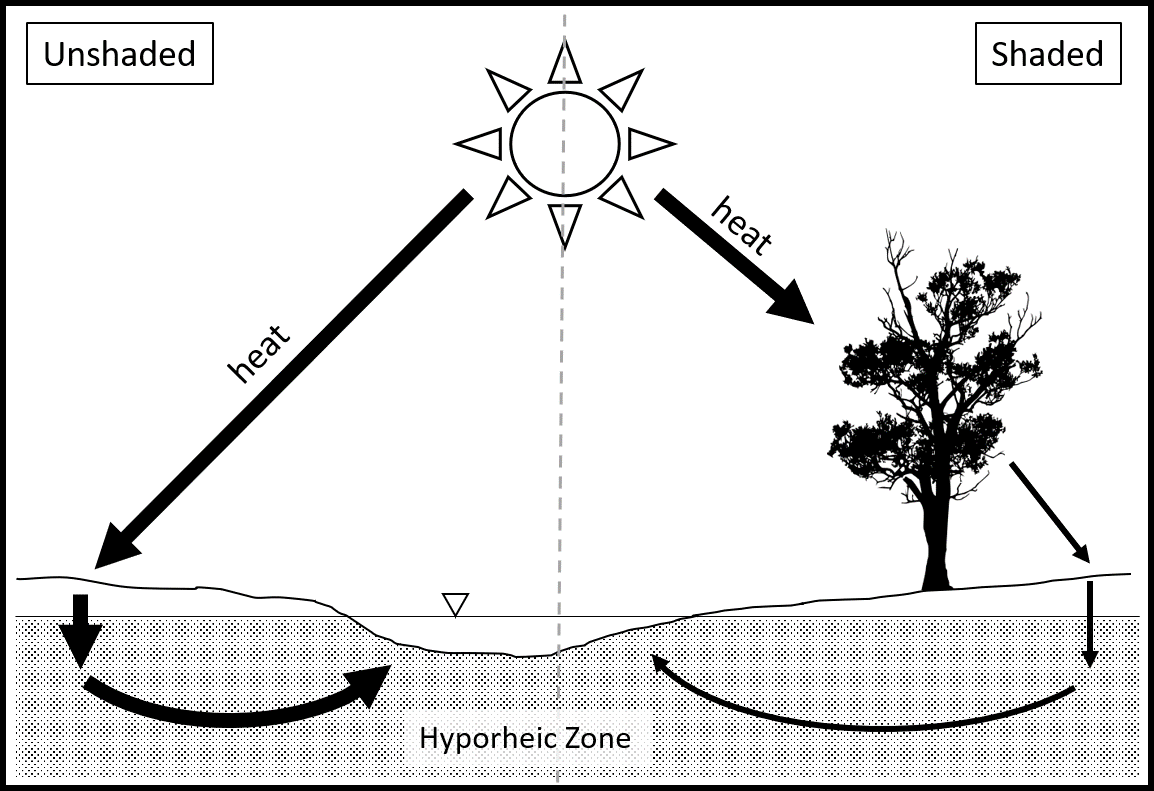
\includegraphics[width=0.4\textwidth]{ShadedAndUnshadedConceptModel.png}
\caption{\label{fig:One} Conceptual model of how shaded and unshaded floodplains alter hyporheic and stream heat dynamics.}
\end{wrapfigure}

Floodplain streams reaches have a unique fluvial landscape where conventional management strategies for reducing stream temperature are largely ineffective. The most common strategy for reducing heat input to a stream is planting stream-bank vegetation to increase channel shade \parencite{Beschta1997RiparianPerspective}. Western floodplain streams have snow-melt dominated hydrology, causing high-energy spring floods which creates an annual scour zone much wider than the summertime base-flow channel \parencite{Whited2007ClimatePattern}. This wide annual scouring prevents young vegetation from reaching maturity and thus prevents the establishment of substantial vegetative shade to the base-flow stream channel.

The vegetation on a floodplain stream reach is rarely close to the base-flow channel, yet the distant floodplain vegetation may indirectly affect stream channel temperatures by protecting shallow hyporheic water from solar radiation (Figure \ref{fig:One}). Prior studies provide indirect evidence for such an effect. Where forests are clear-cut outside of riparian buffer strips, researchers have documented subsequent stream channel warming despite shade from the intact riparian canopy \parencite{Moore2005RiparianReview, Cole2013InfluenceOregon}. Such effects are attributed to the heating of shallow subsurface water from the increased solar radiation in the clear-cut beyond the riparian buffer \parencite{Moore2005RiparianReview, Brosofske1997HarvestingWashington}. However, there are no studies that specifically address how variation in floodplain shade might affect hyporheic water temperature and associated stream channel temperature response (Figure \ref{fig:One}). 



\subsection*{Question}
How does floodplain shade alter hyporheic water temperatures? Additionally, how does the saturated hydraulic conductivity and depth to water table (i.e. thickness of unsaturated floodplain sediment) alter the effects of floodplain shade on hyporheic temperatures?

%How does the interaction of floodplain shade, depth to water hyporheic water table, and saturated hydraulic conductivity alter hyporheic water temperature? 

\subsection*{Hypothesis}
I hypothesize that floodplain shade influences hyporheic temperatures by reducing solar radiation on the ground surface, thereby reducing the conduction of heat through the floodplain sediments overlying the hyporheic zone.

%Heat exchanges between the atmosphere, unsaturated sediments and saturated sediments of a floodplain alter hyporheic water temperatures via conduction of heat through the unsaturated gravels of the floodplains.
%Shading of floodplain sediments overlying lateral hyporheic water leads to less conduction of heat from the sediments to the hyporheic zone and therefore reduces temperatures in the hyporheic zone. 

\subsection*{Prediction}
A modeled floodplain with a cooler soil surface boundary temperature (representing floodplain shade) will result in cooler hyporheic water temperatures relative to a model floodplain with a warmer soil surface boundary (representing a sunny floodplain). The relationship between floodplain shade and hyporheic temperatures will be mediated by the thickness of the overriding sediments -- more pronounced shade effect in shallow hyporheic zones and less pronounced effects in deep hyporheic zones. Additionally, the saturated hydraulic conductivity of the hyporheic zone alters the mean lateral velocity, where the smaller hydraulic conductivity value causes slower hyporheic flow velocity, and the effects of the floodplain surface will be greater.

%\begin{wrapfigure}{L}{0.5\textwidth}
%\centering
%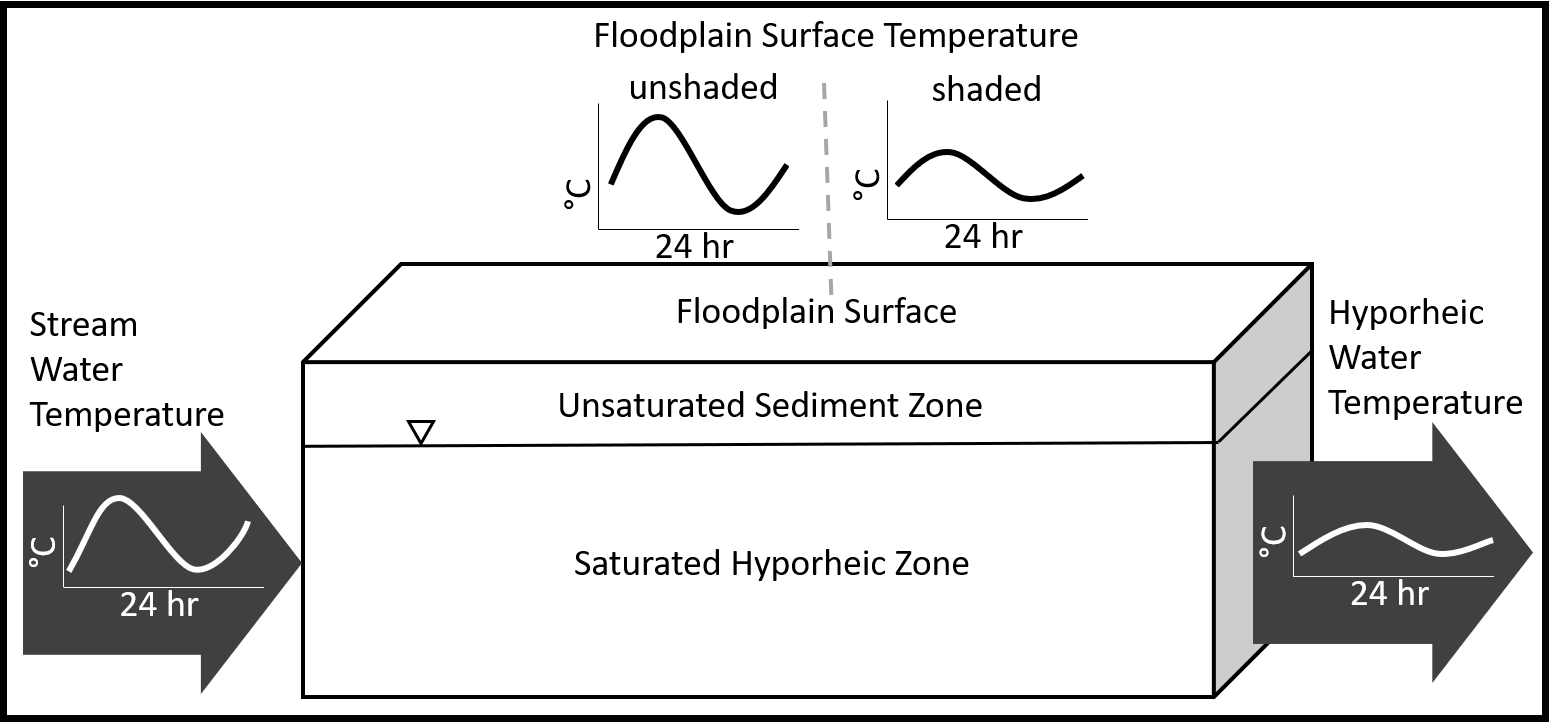
\includegraphics[width=0.5\textwidth]{ModelConceptualModel.png}
%\caption{\label{fig:Two} Diagram of proposed model. Floodplain surface has temperature of either an unshaded or shaded gravels. Stream temperature is input and hyporheic temperature is output.}
%\end{wrapfigure}


%Shading the floodplain sediments reduces conduction of heat through the unsaturated sediment to the hyporheic zone, thus resulting in cooler hyporheic water temperatures when compared to an unshaded floodplain. Also, as the unsaturated sediment layer thickness increases, there will be less of an effect from floodplain shade on hyporheic water temperatures.

\subsection*{Approach}
To simulate hyporheic water flow and heat exchanges, I will use the groundwater model HydroGeoSphere (HGS), which simulates variably-saturated groundwater flow and transport of heat in three dimensions using advective-dispersive porous media transport \parencite{Brunner2012HydroGeoSphere:Model}. Specifically, I will simulate heat transfer in saturated and unsaturated sediments of a single-sided, cross-sectional slice of an idealized floodplain.  The upstream model boundary represents the interface where stream water downwells into the hyporheic zone with a steady-state hyporheic flow rate driven by a 1\% slope -- a topographic grade typical of a montane alluvial floodplain (Figure \ref{fig:Two}). Water entering the hyporheic zone will have daily and annual temperature variation. I will run contrasting model scenarios in which the modeled floodplain surface has temperatures representative of either shaded or sunny floodplain gravels. I will conduct a sensitivity analysis where I vary the thickness of the overlying unsaturated sediments and the saturated hydraulic conductivity of the hyporheic zone for shaded and sunny model scenarios.

For each floodplain scenario, the model will write temperature output across the entire model domain every 15 days across one annual cycle. The output shows how temperature changes along a representative hyporheic flow path, with depth into the unsaturated and saturated zones, and how the spatial patterns change across time. 

%The groundwater model HydroGeoSphere (HGS) will be used to simulate hyporheic water flow and heat exchanges within the hyporheic zone and between the saturated hyporheic zone, unsaturated gravel layer and atmosphere. HGS simulates variably saturated groundwater flow and transport of solutes in three dimensions using advective-dispersive solute transport in porous media \parencite{Brunner2012HydroGeoSphere:Model}. 

%The model domain will be a rectangle set on a 1\% slope. An unsaturated layer will be on top of a saturated layer with constant head at the upstream and downstream boundaries. The temperature of incoming water will be an idealized stream channel temperature signal representative of daily and annual temperature patterns. The boundary top of the unsaturated layer will have an idealized temperature signal representative of shaded or unshaded soil temperatures. The maximum soil temperature of the unshaded signal is from observed summertime gravel temperatures of the Umatilla River floodplain in Pendleton, Oregon, where the minimum daily temperatures are estimated from minimum air temperature of a weather station also on the Umatilla River.

%A sensitivity analysis will be conducted which varies unsaturated layer thickness and degree of floodplain shade. The model will be run for 10 years before outputting groundwater and unsaturated layer temperatures across the entire model domain for 4 days representing each season across the year. This will allow us to understand the effects of floodplain shade and unsaturated layer thickness during different times of year. 

%To address my proposed hypotheses, I will conduct simulation modeling experiments to investigate how floodplain shade influences the interactions among atmospheric heating of floodplain sediments, hyporheic heat transport, and heat exchange between the hyporheic zone (HZ) and channel. 


%From hypothesis 1, I predict that modeled summertime solar radiation loads will warm hyporheic water resulting in greater heat transfer from the HZ to the channel under unshaded conditions and, thus, higher mean daily water temperatures. 


%In real floodplains, the thickness of the unsaturated layer overlying the saturated hyporheic zone varies. Therefore, a sensitivity analysis varying the unsaturated layer thickness and the degree of floodplain shade will be conducted in order to understand their effects on hyporheic temperatures.

%unsaturated layer thickness and shade on a floodplain.

%I will conduct a sensitivity analysis to understand the effects of floodplain conditions on hyporheic water temperatures. I will vary the thickness of the unsaturated layer of floodplain sediments overlaying the hyporheic zone, vary the solar radiative load on the surface of the unsaturated gravels which represents the level of shade on the floodplain, and vary the thickness of the saturated hyporheic zone.  

\section{Effects of floodplain shade on stream channel temperatures via hyporheic water}

In expansive, coarse-grained floodplains, hyporheic zones exchange substantial amounts of water with the stream channel \parencite{Stanford1993AnCorridor, Faulkner2012HyporheicAttributes}, influencing channel water temperature \parencite{Arrigoni2008BufferedChannels, Evans1998}. If shade from floodplain vegetation alters hyporheic water temperatures, rates of hyporheic heat exchange and associated channel water temperatures will be affected. 

Meacham Creek near Pendleton, Oregon underwent a stream restoration in 2011 which significantly altered a section of its floodplain. Meacham Creek flows south to north through a laterally confining valley in the Blue Mountains, where nearly the entire valley width is often considered part of the creek's annual floodplain. The creek's alluvial aquifer is coarse-grained, basaltic gravels and is approximately 3 meters thick. A rail road right-of-way was built along the east valley wall in the early 1900s and portions of Meacham Creek were subsequently dredged against the west valley wall to decrease possible damage to the rail line. 

In 2011, a previously dredged, 1.6 km reach of Meacham Creek was restored back to its natural floodplain and allowed to flow in the middle of the valley. One of the goals of this restoration was to increase hyporheic exchange in an attempt to decrease summertime longitudinal warming in the channel. However, in the summers after the restortation, the longitudinal warming increased. As a consequence of constructing the new stream channel, much of the floodplain forest was cut down, thus decreasing the amount of shade on the floodplain. Additionally, the amount of stream-side shading on the channel itself was approximately the same pre- and post-restoration. Thus, I hypothesize that the decrease in floodplain shade increased solar radiation on the floodplain, warming hyporheic water, which upon upwelling back to the stream channel caused increased longitudinal warming. 

Riparian deforestation is not often caused by a ``noble" practice such as stream restoration, rather riparian deforestation is more commonly caused by human development, forest harvesting and wildfire. In an effort to protect streams from degraded water quality caused by riparian deforestation, federal and local agencies require a specified width of riparian forest to remain intact lateral to the stream channel. In practice, this riparian ``buffer" width is often measured from the stream-bank margin. This datum poses a problem for gravel-bedded floodplain reaches with snow-melt dominated hydrology because stream-bank margins tend to move annually and can significantly change depending on the time of year (summertime base-flow versus springtime flood-peak). Additionally, hyporheic zones of floodplains are usually very wide and the prescribed riparian buffer width may not encompass the full width of interaction between the stream channel and alluvial aquifer. When the riparian forest is reduced above this area of interaction between the stream channel and hyporheic zone, the increase in solar radiation has the potential to warm hyporheic water, which may cause warming of the stream channel. 

I predict that the degree to which floodplain shade -- or lack thereof -- influences stream channel temperatures is highly dependent on the spatial distribution of vegetation and hyporheic flow paths. Shading longer hyporheic flow paths will likely have more of an influence on hyporheic temperatures than shading shorter ones. Water downwelling into the hyporheic zone is the same temperature as the stream channel, and if the water upwells back to the channel relatively quickly, the temperature is still relatively similar to the channel temperature. At longer flow paths, the temperature of hyporheic water changes due to diffusion and dispersion of heat between the water and alluvium and among water parcels of different temperatures. The longer a water parcel is in the hyporheic zone, the more it will be influenced by heat exchanges within the hyporheic zone and between the hyporheic zone and it surroundings -- thus, if the unsaturated sediments above the hyporheic zone are warmed considerably via solar radiation, the hyporheic water will exchange more heat with this warm layer right above it. 

However, when considering these longer flow paths which have been warmed by ground-surface solar radiation, their influence on stream temperature may be insubstantial because a common assumption of hyporheic residence times (and flow path lengths) is that they have a power-law shaped frequency distribution. This power-law residence time distribution means that most hyporheic water upwells back to  he channel after a short period of time (and short flow path length) and very little water upwells from long flow paths -- where the effects of floodplain shade may be most pronounced. I predict that there is an optimum, intermediate flow path length where the effects of shade have the greatest effects on stream channel temperatures. This intermediate flow path length is long enough to where heat exchange with the overlying floodplain sediments causes a notable change in hyporheic temperature and enough water from this flow path length upwells back to the channel to cause a notable change in stream channel temperature.

\subsection*{Question}
%To what extent does vegetation on a floodplain lateral to a stream channel affect heat dynamics in the hyporheic zone and in the channel of a real stream reach?
How does the spatial variability in floodplain shade and hyporheic flows interact to influence water temperatures in a stream channel?

\subsection*{Hypothesis}
%Where shade occurs on a floodplain in relation to hyporheic flow path location and direction has a variable influence on hyporheic water temperatures, thus the distribution of water temperatures in the channel depends upon the spatial attributes of shade and hyporheic exchange in the floodplain. 

The spatial juxtaposition of shade and hyporheic flow paths on the floodplain govern the exchange of heat between the atmosphere, hyporheic zone, and channel, ultimately determining the magnitude of channel temperature response.


\subsection*{Prediction}
Floodplain shade, hyporheic flow path length and direction interact to influence the distribution of water temperatures upwelling to the stream channel. When more floodplain shade occurs, upwelling water temperatures will be cooler, whereas when there is little to no floodplain shade, upwelling water will be warmer, thus altering the temperature regime of the channel. I predict that shading in certain areas of the floodplain have a larger influence on stream channel temperatures than other areas of the floodplain. These locations of greatest influence will occur where intermediate and long hyporheic flow path lengths occur. Floodplain shade will have little influence at locations where shorter hyporheic flow paths are because this short lived hyporheic water does not spend enough time in the hyporheic zone for vertical conduction to cause a significant change in temperature. Additionally, the influence on stream temperatures will depend on the residence time distribution of upwelling hyporheic water. In hyporheic zones with power-law residence time distributions shifted toward shorter flow paths, the influence of floodplain shade will be less than in hyporheic zones with residence time distributions shifted toward longer flow paths. 


%Long flow paths will be influenced greatly from floodplain shade, but if assuming a power-law residence time distribution in the hyporheic zone, long flow path 

%A spatially explicit model of pre-restoration floodplain vegetation will show less heat input to the channel from hyporheic exchange than a model with post-restoration floodplain vegetation. Post-restoration will show more heat input from the hyporheic zone to the channel. 
%Comparison of stream heat budgets using pre-restoration floodplain vegetation levels to post-restoration vegetation levels will show an increase in heat coming from hyporheic exchange.

%Early port-restoration = more heat coming from the floodplain
%Current vegetation levels = less heat coming from the floodplain
%Pre-retoration vegetation levels = much less heat coming from floodplain


%A groundwater heat model with minimal, post-restoration floodplain shade will have warmer hyporheic and stream temperatures than the same model with floodplain shade at high vegetation levels similar to pre-restoration.  

\subsection*{Approach}
The groundwater model HydroGeoSphere (HGS) will be used to simulate stream and hyporheic water flow along with heat exchange across the entire model domain. I will use the 1.6 km Meacham Creek restoration site as the model stream. The HGS model grid will be set up using elevation rasters of Meacham Creek collected using LiDAR in 2013 such as the model depicted in Figure \ref{fig:Three}. The lowest, bare-earth elevations will be used to parameterize the stream flow and head gradients in the hyporheic zone. The highest hits raster will be used to characterize the vegetation on the floodplain and simulate the shade pattern on the floodplain surface. 

\begin{wrapfigure}{L}{0.5\textwidth}
\centering
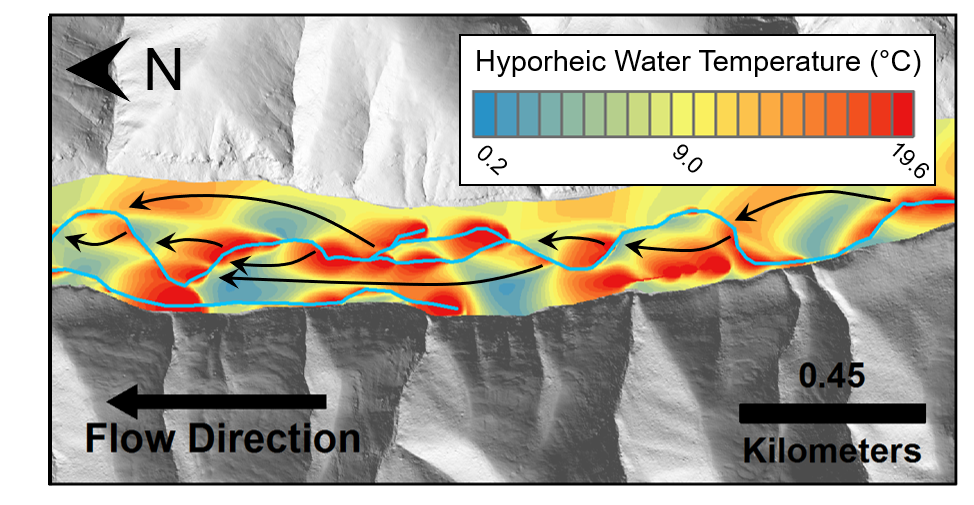
\includegraphics[width=0.5\textwidth]{HyporheicModel.png}
\caption{\label{fig:Three} Output from HGS model describing summertime subsurface HZ temperatures on the Meacham Creek floodplain, OR (B. Amerson, \textit{unpublished data}). Blue line depicts channel location; black arrows trace example hyporheic water movement.}
\end{wrapfigure}


Floodplain shade is a spatial variable and will be modeled to create a boolean shade raster. To categorize floodplain shade on Meacham Creek, the method of \cite{Loicq2018ImprovingData} will be used. This method uses geometric principles and LiDAR data to determine which raster cells have shade cast on them for a certain date and time. The LiDAR data was taken post-restoration, therefore shade density will be estimated from satellite imagery pre-2011.

The following model scenarios of the Meacham Creek floodplain will be compared: 
\begin{enumerate}
    \item Full sun, no vegetation control
    \item Full shade control
    \item Post-restoration floodplain vegetation
    \item Pre-restoration floodplain vegetation
\end{enumerate}

In order to isolate the effects of shade on the floodplain and not the shade on the stream itself, I will standardize the solar radiation input to the stream surface across all model scenarios. It is already well understood that shading on the stream surface cools stream temperature, thereby confounding the effect of floodplain shade if we include stream surface shade. 

In order to fully  understand the potential effects of floodplain shade on stream water temperature, beyond a site-specific investigation of Meacham Creek, I will use Monte Carlo methods to randomly distribute vegetative shade across the floodplain.



%To address hypothesis 2, I will model the Meacham Creek floodplain, Pendleton, Oregon. A 1.6 km reach of this floodplain underwent a restoration that increased hyporheic exchange but also greatly decreased the amount of shade on the floodplain. The floodplain will be modeled in HGS using LiDAR raster data such as the model depicted in Figure \ref{fig:Three}. This model depicts temperatures in the hyporheic zone, but did not simulate heat exchange across the floodplain surface to the hyporheic zone. The ``highest hits'' LiDAR data represents tree height, and shade on the floodplain will be modeled using this data along with sun angle geometry to calculate the heat exchange between the floodplain surface and hyporheic zone. This spatially explicite model allows us to understand where the spatial location of shade and hyporheic flow paths have the greatest effect on temperature. I predict that floodplain shade will have the greatest effect on hyporheic flow paths that are both shallow and long. 


\section{Scaling hyporheic heat exchange dynamics to whole stream temperature regimes} 

The transfer of mass (i.e. water) with a certain temperature is a heat exchange
advection- transfer of heat along with the transfer of mass

"Heat convection occurs when bulk flow of fluid (gas or liquid) carries heat along with the flow of matter in the fluid."
"All convective processes also move heat partly by diffusion, as well"
"Advection is sometimes confused with the more encompassing process of convection which is the combination of advective transport and diffusive transport"
"More technically, convection applies to the movement of a fluid (often due to density gradients created by thermal gradients), whereas advection is the movement of some material by the velocity of the fluid."

When talking about heat, we don't need to talk about "dispersion" - that term should only be used for mass transfer of a substance. Diffusion is the correct term of heat transfer.

In streams overlying expansive, coarse-grained alluvial aquifers, hyporheic exchange can potentially influence the temperature dynamics in the stream channel. The extent of this influence is determined by the gross water exchange with the hyporheic zone and the heat fluxes within the hyporheic zone. The heat transfer processes occurring within the hyporheic zone include advection -- heat transferred along with the bulk movement of the water,  and diffusion -- the spreading of heat caused by a concentration gradient. 

In these stream systems, with high rates of hyporheic exchange, there is a tremendous amount of bulk water movement between the stream channel and the hyporheic zone,

\subsection*{Question}
At what scales are advection and dispersion of heat in the hyporheic zone important for simulating heat exchange in the hyporheic zone and between the hyporheic zone and channel?

How do the processes of advection and dispersion of heat, components of hyporheic heat exchange, scale from reach to whole stream? And how can a simplified perspective on advective and dispersive heat exchanges  be represented based on a power-law hyporheic residence time distribution?

%How do we represent advection and dispersion in a quasi-1D setting in order to simulate the overall effect of hyporheic heat transfer and storage on whole channel temperature regimes?

\subsection*{Hypothesis}
Advective transport of heat, rather than dispersion, is the dominant process of heat exchange between the stream channel and hyporheic zone in expansive, coarse-grained alluvial aquifers and that representation of advection alone (along with numerical dispersion) in a heat exchange model is able to simulate the effects of hyporheic exchange on stream channel temperatures.

\subsection*{Prediction}
If the dominance of advective transport processes is sufficient, we predict that heat budgets that ignore dispersive heat transport will provide accurate estimates of the effects of hyporheic heat exchange on stream channel temperature dynamics. Conversely, if dispersive heat transport represents a sufficiently important mechanism of heat transfer, we expect inaccurate estimates of stream temperature dynamics that will require either modification to parameters in our advection-only TempTool model or adjustment in the underlying model assumptions and structure to incorporate dispersive heat exchanges.


%TempTool will underestimate the amount of damping and lagging occurring at long residence times because it currently has a constant rate of dispersivity. 


\subsection*{Approach}
We will use both HydroGeoSphere and TempTool (a simplified, quasi-1-dimensional model of stream channel and hyporheic temperature; a prior product of this project) to create heat budgets of the Meacham Creek alluvial aquifer. HGS is an established and verified model that calculates both advective and dispersive heat exchanges in an alluvial aquifer to generate a river channel heat budget. However, the detailed nature of its parameterization requirements prevents application of HGS at the scale of 10s of km of river corridor. 

TempTool integrates advective heat exchange between the river channel and hyporheic zone, along with advective heat transport through and heat storage within the hyporheic zone into a river channel heat budget.  Its novel approach is relatively untested, but as a 1D model with minimal required parameters, it can operate at the scale of 10s of km of river length.  We will compare heat budgets predicted by HGS and TempTool to determine the relative importance of dispersive vs. advective heat transport in coarse-grained alluvial aquifers, and develop strategies for parameterizing TempTool’s advection-only strategy to incorporate dispersive heat flux. 

Generally, we will be comparing the HGS hyporheic temperatures to the TempTool hyporheic temperatures across the same residence times to get at estimate of how well TempTool is at estimating the correct amount of temperature buffering and lagging. This will help us better understand the mechanisms by which heat moves in the hyporheic zone. 
%Based on whether or not TempTool is accurate at this estimation, we will modify and adjust the model to account for the change in dispersivity or any other error that comes up in this modeling exercise.   


\printbibliography
\end{document}
